\title{PNG (Portable Network Graphics)}

\maketitle
\tableofcontents

\section{Posibilities}
\begin{itemize}
\item \url{http://www.libpng.org/pub/png}.
\item Fully lossless.
\item Only raster (not vectorized) images.
\item Better funtionality and performance than GIF (Graphics
  Interchange Format), that uses an patented implementation of the LZW
  algorithm, and TIFF (Tagged Image File Format).
\item Free usage and free from patents.
\item Palletized images (up to 256 colors), true color images (up to
  48-bits/pixel) and grayscale images (up to 16-bits/pixel).
\item On-the-fly encoding and decoding (streamability).
\item Alpha channels (variable transparency).
\item Gamma correction (cross-platform control of image brightness).
\item Progressive and interlazed images.
\item Progressive reconstructions by means of spatial scalability.
\end{itemize} 

\section{Codec}
\begin{center}
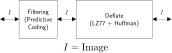
\includegraphics[width=20cm]{PNG_codec_ext}
\end{center}

\section{Filtering (encoding)}
\begin{itemize}
\item Optional.
\item Predictive encoder that reduces the spatial correlation.
\item Pixels are translated to prediction residues (errors):
  \begin{displaymath}
    E = X - \hat{X}
  \end{displaymath}
  where $X$ is the pixel-value and $\hat{X}$ its prediction.
\item The entropy of the residue image is typically smaller than the
  original image's one, and the residues follow a Lapace probability
  distribution, centered in 0 (the average of the prediction error is
  0).
\item Available predictors (``filters''):
  \begin{center}
    \begin{tabular}{cc}
      \begin{tabular}{rcl}
        Type & Predictor & Prediction \\
        \hline
        0 &	None 	& $\hat{X}\leftarrow 0$ \\
        1 &	Sub 	& $\hat{X}\leftarrow A$ \\
        2 &	Up 	& $\hat{X}\leftarrow B$ \\
        3 &	Average & $\hat{X}\leftarrow (A+B)/2$ \\
        4 &	Paeth 	& $\hat{X}\leftarrow A + B - C$
      \end{tabular}
      &
      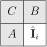
\includegraphics[width=3cm]{contexto_prediccion}
    \end{tabular}
  \end{center}
\item The predictor can be changed in the middle (of the encoding) of
  an image.
\end{itemize}

\section{``Deflate'' (encoding)}
\begin{itemize}
\item It's a generic text-compression algorithm based on LZ77 and
  Huffman and written by Jean-loup Gailly and Mark
  Adler\footnote{Authors of The Data Compression Book
    \cite{Nelson96}}.
\item LZ77 removes the statistical redudancy of high order (remember
  that the preditor has removed the spatial redundancy).
\item The Huffman encoder removes the statisctical redundancy of order
  0. The probabilistic model used is adaptive and initially empty.
\end{itemize}

\section*{The PPM (Portable aNyMap) container}
% \begin{verbatim}
% struct PGM_image {
%   "P5\n",        /* Magic number */
%   char width[],  /* Columns */
%   "\n",
%   char height[], /* Rows */
%   "\n",
%   char depth[],  /* 2^number_of_bits_per_component */
%   "\n",
%   if depth == "255" {
%     unsigned char pixel[width][height];
%   } else if depth == "65535" {
%     unsigned short pixel[width][height];
%   }
% };
% \end{verbatim}

% \newpage
\begin{verbatim}
struct PPM_image {
  "P6\n",        /* Magic number */
  char* width, " ", height,  /* Columns and rows */
  "\n",
  char* depth,   /* 2^number_of_bits_per_component */
  "\n",
  struct RGB_pixel pixel[width][height];
}

if (depth == "255") {
  struct RGB_pixel {
    unsigned char R;
    unsigned char G;
    unsigned char B;
  }
} else if (depth == "65535") {
  struct RGB_pixel {
    unsigned short R;
    unsigned short G;
    unsigned short B;
  }
}
\end{verbatim}

% \section*{Let's go to the lab!}
% \begin{itemize}
% \item Use the \texttt{pnmtopng} tool for encode the sequences of
%   \href{http://www.hpca.ual.es/~vruiz/videos/}{the Test Video
%     Corpus}. Notice that each frame must be in PPM format.
%   \begin{flushleft}
%     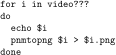
\includegraphics[width=0.4\textwidth]{akiyo_compresion_PNG}
%   \end{flushleft}
% \item Fill the table: 
% \begin{verbatim}
% Codec | akiyo mobile parkrun stockholm Average
% ------+---------------------------------------
%   PNG | 
% \end{verbatim}
% \item What's about the temporal scalability?
% \end{itemize}

\section*{Let's go to the lab!}
\begin{itemize}
\item Use the \texttt{pnmtopng} command line tool to fill the table:
\begin{verbatim}
   Codec | lena boats pepers zelda Average
---------+--------------------------------
pnmtopng | 
\end{verbatim}
\end{itemize}

\bibliography{text-compression}
